\providecommand{\econtexRoot}{}
\renewcommand{\econtexRoot}{..}
% The \commands below are required to allow sharing of the same base code via Github between TeXLive on a local machine and ShareLaTeX.  This is an ugly solution to the requirement that custom LaTeX packages be accessible, and that ShareLaTeX seems to ignore symbolic links (even if they are relative links to valid locations)
\newcommand{\econtex}{\econtexRoot/texmf-local/tex/latex/econtex}
\newcommand{\econtexSetup}{\econtexRoot/texmf-local/tex/latex/econtexSetup}
\newcommand{\econtexShortcuts}{\econtexRoot/texmf-local/tex/latex/econtexShortcuts}
\newcommand{\econtexBibMake}{\econtexRoot/texmf-local/tex/latex/econtexBibMake}
\newcommand{\econtexBibStyle}{\econtexRoot/texmf-local/bibtex/bst/econtex}
\providecommand{\EqDir}{\econtexRoot/Equations}
\providecommand{\FigDir}{\econtexRoot/Figures}
\providecommand{\CodeDir}{\econtexRoot/Code}
\providecommand{\CodeDir}{\econtexRoot/Data}
\providecommand{\SlideDir}{\econtexRoot/Slides}
\providecommand{\TableDir}{\econtexRoot/Tables}
\providecommand{\ResourcesDir}{\econtexRoot/Resources}
%\providecommand{\ApndxDir}{.} % Appendices can be in a subdirectory (and this can be redefined to, say, \providecommand{\ApndxDir}{\econtexRoot/Appendices} only if they do not reference any resources (Tables, Equations, Code, etc) in any other directory

  
\documentclass[titlepage,letterpaper]{\econtex}

\providecommand{\texname}{FlawedPaper}
\usepackage{vmargin}
\usepackage{float}
\usepackage{\econtexSetup}\usepackage{\econtexShortcuts}

\usepackage[en-US]{datetime2}\DTMlangsetup{showdayofmonth=true} 

\provideboolean{ifWeb}\setboolean{ifWeb}{false}\opt{Web}{\setboolean{ifWeb}{true}}

\ifthenelse{\boolean{ifWeb}}{\usepackage{grfext} 
  \PrependGraphicsExtensions*{.svg,.jpg,.JPG,.png,.PNG,.pdf,.PDF}
}{} 

\providecommand{\versn}{} 
\ifthenelse{\boolean{ifWeb}}{  \renewcommand{\ushort}{\underline}\renewcommand{\versn}{Web} }{} 

\newboolean{verbatimwriteOn}   

\setboolean{verbatimwriteOn}{false} 
\newcommand{\ifVerbatimWrite}{\ifthenelse{\boolean{verbatimwriteOn}}} 
\ifVerbatimWrite{}{
  \renewenvironment{verbatimwrite}[1]{} 
} 

\newenvironment{Private}{} 

\providecommand{\wAlt}{\omega}
\providecommand{\sConst}{\varsigma}

\newtheorem{defn}{Definition}
\newtheorem{theorem}{Theorem}
\newtheorem{lemma}{Lemma}
\newtheorem{corollary}{Corollary}
\newtheorem{prop}{Proposition}

\renewcommand{\cite}{\citeyear}

\setmarginsrb{1in}{1in}{1in}{1.4in}{0pt}{0pt}{0pt}{.3in} 

\provideboolean{bigdouble}    
\setboolean{bigdouble}{true} 
\setboolean{bigdouble}{false} 

\ifthenelse{\boolean{bigdouble}}{ 
  \setmarginsrb{0.40in}{0.8in}{0.40in}{0.8in}{0pt}{0pt}{0pt}{0.2in} 
}{} 

\begin{document}\bibliographystyle{\econtexBibStyle}

%\hfill{\tiny \texname~\versn~\today~{at} \DTMcurrenttime, \input{.git-source-commit}~~\input{.git-public-commit}}

\title{An Attempt at the Replication of \\ Yongsung Chang and Sun Bin-Kim's \\ Heterogeneity and Aggregation: \\ Implications for Labor-Market Fluctuations}

\newlength\TableWidth

\ifthenelse{\boolean{ifWeb}}{
  \author{
   Wonsik Ko \authNum
    \and
    Syareza Tobing \authNum
  }
}{
  \author{
   Wonsik Ko\authNum \\ {\small Johns Hopkins University}
    \and
   Syareza Tobing\authNum \\ {\small Johns Hopkins University} 
  }
} 

\date{December 22, 2020}
\maketitle

\jelclass{D31, E32, J22, J24, J31\\
  \href{https://econ-ark.org}{
\includegraphics{./Resources/PoweredByEconARK}} \\ \phantom{.}}

\keywords{optimal consumption and labor, heterogeneous-agents, incomplete capital markets, indivisible labor}


\hypertarget{Abstract}{}
\begin{abstract}
This paper adresses the low correlation between hours and productivity in the business cycle literature along with the large cyclical movement in the wedge derived for the intratemporal choice of commodity consumption and hours worked in the business cycle literature. Using only a technology shock as the aggregate disturbance, the authors obtained a low correlation between hours worked and productivity. The interaction between incomplete capital markets and indivisible labor breaks the link between employment and wages at the aggregate level. Aggregate employment is not highly correlated with productivity because individual optimality conditions do not aggregate well.
\end{abstract}

\vspace{-1cm}
\begin{authorsinfo}
  \name{Ko: Department of Economics, Johns Hopkins University, email: \href{mailto:wko5@jhu.edu}{\texttt{wko5@jhu.edu}}}
  \name{Tobing: Department of Economics, Johns Hopkins University, email:  \href{mailto:mtobing1@jhu.edu}{\texttt{mtobing1@jhu.edu}}}
\end{authorsinfo}

\hypertarget{links}{}
\medskip
\begin{small}
  \parbox{\textwidth}{
    \begin{center}
      \begin{tabbing}
        \texttt{Original Papper:~} \= \= \texttt{\href{https://www.aeaweb.org/articles?id=10.1257/aer.97.5.1939}{American Economic Association (Paywall)}} \\
        \texttt{~~~GitHub:~} \> \> \texttt{\href{https://github.com/raytobing/final_project/tree/master/replication}{Replication Project}} \\
      \end{tabbing}
    \end{center}

  } 
\end{small}

\titlepagefinish

\setcounter{page}{1}

\setcounter{footnote}{0}

\ifthenelse{\boolean{ifWeb}}{\thankstext}{}

\hypertarget{Introduction}{}
\section{Introduction}\label{sec:Intro}

\begin{verbatimwrite}{./Sections/Intro.tex}

\subsection{Goal}\label{sec: Goal}

The goal of this project is to replicate the main results from \citet{changkim2007} using the tools provided by HARK. We use the  infrastructure provided by the Krusell-Smith Replications or Reproductions (REMARK) provided by the econ-ark project and attempt to extend it to include the specifications written by Chang and Kim.
  Ultimately, we would like to completely replicate the results shown in Figure \ref{fig:goal}, specifically the third line as written in the legend box, which is the Labor-Market wedge obtained from a model with incomplete capital markets and indivisible labor supply. 

  \begin{figure}[ht]
    {\centering \includegraphics[width=.95\textwidth]{\FigDir/figure_5.pdf}}
    \caption{Labor-Market Wedges From The Models}
    \label{fig:goal}
  \end{figure}

  Given our current limitations and lack of familiarity with HARK, we have decided to forgo replicating the model with incomplete capital market and indivisible labor supply and instead attempt the more achievable goal of replicating the model with an incomplete market and divisible labor supply.
  The main body of this paper will provide a summary of the original paper and go through some of the results produced by their simulation. Subsequently, the Appendix will show what we have managed to producce using HARK along with a brief explanation of the method we used to extend the tools currently available in HARK to accommodate the replication of Chang and Kim's results. For a more thorough elaboration of this process, we have made the annotated code that produces the replication publicly available on our GitHub page.

  \subsection{Error in the Original Paper}\label{sec: Error}

  Following the publication of the original paper by Chang and Kim, \citet{Takahashi2014comment} showed that the results produced by Chang and Kim arise from errors in their computational method. Takahashi then resolved their model using a corrected method and found a strong, positive correlation between hours and productivity.
  This error raises the importance of reproducibility in economics and science in general. Given the increasing complexity of methods used in economic research, there is a dire need of a general tool such as HARK  to ensure that errors are quickly identifiable and are caught early in the publication process rather than being found seven years after publication.

\subsection{The Problem}\label{sec: The Problem}

  $$U(C_t , H_t) \ = \ lnC_t \ - \ B \bigg[ \frac{H^{1+1/\gamma}}{(1 \ + \frac{1}{\gamma})} \bigg]$$

\begin{align*}
C_t \    &: \text{commodity consumption}\\
H_t \    &: \text{hours worked}\\
\gamma \ &: \text{compensated labor supply elasticity}\\
B \      &: \text{constant}
\end{align*}
  
 Assuming an aggregate Cobb-Douglas production function with labor-income share denoted by $\alpha$, the Marginal Rate of Stubstitution (MRS) should be equal to the Marginal Productivity of Labor (MPL):

 $$B \frac{H_t^{1/\gamma}}{C_t^{-1}} \ = \ \alpha \frac{Y_t}{H_t}$$

 Nevertheless, as we can see from Figure \ref{fig:mrs_prod} below, the MRS is more volatile than hours and often moves in opposite direction to productivity, thereby violating the equilibrium.

 \begin{figure}[H]
   \centering
   \includegraphics[scale=.22]{\FigDir/figure_1.pdf}
   \caption{Cyclical Components of MRS and Labor Productivity}
    \label{fig:mrs_prod}
  \end{figure}

On the other hand, the labor-market wedge is defines as:
$$ln \ Wedge_t \ = \ ln \ MRS_t \ - \ ln\frac{Y_t}{H_t} \ + \ constant$$

     \begin{figure}[H]
   \centering
   \includegraphics[scale=.22]{\FigDir/figure_2.pdf}
   \caption{Cyclical Components of Hours and Labor-Market Wedge for The United States}
    \label{fig:wage_hours}
  \end{figure}

Subsequently, Figure \ref{fig:wage_hours} shows that the wedge is highly correlated with hours worked and its volatility has similar magnitude as hours worked. The wedge arises because hours worked are not highly correlated with productivity.

\end{verbatimwrite}\ifVerbatimWrite{\input{Sections/Intro}}{}

\hypertarget{Model}{}
\section{The Model}\label{sec:Model}

\begin{verbatimwrite}{./Sections/Setup-Intro}

\subsection{Setup}\label{sec:Setup}  

The model is an extension of \citet{KrusellSmith1998}'s heterogeneous agent model with incomplete capital markets (\citet{Aiyagari1994}) to indivisible labor supply (\citet{Rogerson1988}). A continuum of workers have identical preferences but different productivity along with a separable preference over consumption and hours worked. Capital markets are incomplete. Workers trade claims for physical capital, $a_t$ that yields a return of $r_t$ Workers face a borrowing constraint $a_t \geq \bar{a},$ for all t. Labor supply is indivisible such that if employed, a worker supplies $\bar{h}$ units of labor and earns $w_t x_t \bar{h}$ where:
\begin{itemize}
    \item $w_t$: wage rate per effective unit of labor
    \item $x_t$: individual productivity
    \end{itemize}

   $w_t$ varies exogenously according to a stochastic process with a transition probability distribution function defined as:
    $$\pi_x(x'|x) \ = \ Pr(x_{t+1} \leq \ x'|x_t \ = \ x)$$
  $x_t$ is the only idiosyncratic risk faced by the agents in the model and the only source of heterogeneity

    Output is produced through a Cobb-Douglas Production function defined by: \\
    $$Y_t \ = \ F(L_t,K_t, \lambda_t) \ = \ \lambda_t L^\alpha_t K^{1-\alpha}_t$$
    \begin{itemize}
        \item $K_t$: capital which depreciates at rate $\delta$ each period
       \item $L_t$: effective units of labor
       \item $\mu$: distribution of workers
       \item $\lambda$: aggregate productivity 
       \end{itemize}

      $\lambda$ evolves with a transition probability distribution function:
           $$\pi_\lambda (\lambda'|\lambda) \ = \ Pr(\lambda_{t+1} \leq \lambda ' | \lambda_t \ = \ \lambda)$$

     The value function for an employed worker is:

     \begin{align*}
      \begin{split}
 V^E (a,& \ x; \ \lambda, \ \mu)\\
 = & \max_{a' \ \in \ A} \bigg\{ ln \ c \ - \ B \frac{h^{1 \ 1/ \gamma}}{1 \ + \ 1/ \gamma}\\
 \\
 & + \ \beta E[max \{ V^E (a',x';\lambda ', \mu'), \ V^N (a',x'; \lambda ', \mu ') \}|x, \lambda] \bigg\},\\
\end{split}
     \end{align*}

     subject to:

 $$c \ = \ w( \lambda, \mu )x \bar{h} \ + \ (1 \ + \ r)\lambda,\mu))a \ - \ a',$$
 $$a' \geq \bar{a},$$
 $$\mu ' \ = \mathbb{T}(\lambda,\mu)$$

        where $\mathbb{T}$ is a transition operator defining the law of motion for the distribution of worker $\mu$. The value function of non-employed worker (h = 0) is defined by:
$$V(a,x; \lambda,\mu) \ = \max_{h \in \{0, \bar{h}\}} \{V^E (a,x; \lambda, \mu), \ V^N (a,x;\lambda,\mu) \}$$

\subsection{Equilibrium Conditions}\label{sec:Equilibrium}

Equilibrium consists of:
\begin{enumerate}
  \item A set of value functions 
  $$ V^E (a,x;\lambda,\mu), \ V^N (a,x;\lambda,\mu), \  V (a,x;\lambda,\mu)$$ 
  \item A set of decision rules for consumption, asset holdings and labor supply 
    $$\{c(a,x;\lambda,\mu), \ a'(a,x;\lambda,\mu), \ h(a,x;\lambda,\mu)\}$$ 
  \item A set of decision rules for aggregate inputs 
    $$\{K (\lambda,\mu),L(\lambda,\mu)\}$$ 
  \item A set of decision rules for factor prices 
    $$\{ w(\lambda,\mu),r(\lambda,\mu)\}$$ 
  \item Law of motion for the distribution of workers 
    $$\mu ' \ = \ \mathbb{T}(\lambda,\mu)$$
  \end{enumerate}

  such that:
  
  \begin{enumerate}
    
\item Individuals optimizes given $w(\lambda,\mu)$ and $r(\lambda,\mu)$.

\item Representative firms maximizes profits.
$$w(\lambda,\mu) \ = \ F_1 (L(\lambda,\mu), K(\lambda,\mu), \lambda)$$
$$r(\lambda,\mu) \ = \ F_2 (L(\lambda,\mu), K(\lambda,\mu), \lambda) \ - \ \delta$$

\item The goods market clears.
$$\int \{ a'(a,x; \lambda, \mu) \ + \ c(a,x; \lambda, \mu)\} d \mu $$
$$= \ F(L(\lambda,\mu), K(\lambda,\mu), \lambda) \ + \ (1 \ - \ \delta)$$

\item Factor market clears.
$$L(\lambda,\mu) \ = \ \int xh(a,x;\lambda,\mu) \ d \mu$$
$$K(\lambda,\mu) \ = \ \int a \ d \mu$$

\item Individual and aggregate behaviours are consistent.
$$\mu ' (A^0 , \ X^0)$$
$$ = \int_{A^0 , X^0} \int_{A,\chi} \mathbbm{1}_{a'=a'(a,x;\lambda,\mu)} d\pi_x (x'|x)d\mu \} da'dx'$$

\end{enumerate}
  
\end{verbatimwrite}\ifVerbatimWrite{\input{Sections/Model}}{}

\section{Quantitative Analysis}\label{sec:QuantAnalysis}

\subsection{Calibration}\label{sec:Calibration}

The unit of time is business quarter and parameters are obtained from the Panel Study of Income Dynamics (PSID) along with the empirical labor supply literature. Parameters are summarized in Table \ref{fig:table_1} below:

     \begin{table}[H]
       \centering
         \includegraphics[scale=0.3]{\FigDir/table_1.pdf}
         \caption{Parameters of the Benchmark Model Economy}
    \label{fig:table_1}
  \end{table}

  \subsection{Cross-Sectional Distribution for Earnings, Wealth and Reservation Wages}\label{sec:CrossSectional}

       \begin{table}[H]
    {\centering \includegraphics[width=.95\textwidth]{\FigDir/table_2.pdf}}
    \caption{Characteristics of Wealth Distribution}
    \label{fig:table_2}
  \end{table}
  
Table \ref{fig:table_2}  summarizes the PSID and the model's information on wealth and earnings. For each quintile group of wealth distribution, the authors calculated:

\begin{enumerate}
\item Wealth share
\item Ratio of group average to the  economy-wide average
\item Earnings share
\end{enumerate}

In the model, labor-market participation is determined by market opportunity (wage) and wealth (asset holdings). The steady-state reservation wage schedule is shown in Figure \ref{fig:figure_3}  below.

\begin{figure}[H]
  \centering
    \includegraphics[scale=0.3]{\FigDir/figure_3.pdf}
  \caption{Reservation Wages From the Benchmark Model}
    \label{fig:figure_3}
  \end{figure}


\subsection{Cyclical Properties of the Model}\label{sec:CyclicalProperties}

The equilibrium of the model is solved using the "bounded rationality" method developed by Krussel Smith (1998) where agents uses a finite set of moments of $\mu$ in forecasting aggregate prices. Table \ref{fig:table_3}  below presents the volatility of key aggregate variables in the model economy.

       \begin{table}[H]
         \centering
         \includegraphics[scale=0.5]{\FigDir/table_3.pdf}
         \caption{Volatilities of Aggregate Variables}
    \label{fig:table_3}
  \end{table}
  

These main observations obtained from Table \ref{fig:table_3} are:
\begin{itemize}
\item Ouput volatility is less than 2/3 of actual output volatility, similar to that of the standard representative agent models.
\item Volatility of hours relative to output and the volatility of labor productivity relative to output is the same as that in the data.
\item The realtive volatility of hours to productivity is very colse to that in the data.
\end{itemize}

Subsequently, Table \ref{fig:table_4}  below shows the cyclicality of key aggregate variables.

       \begin{table}[ht]
         \centering
         \includegraphics[scale=0.5]{\FigDir/table_4.pdf}
         \caption{Volatilities of Aggregate Variables}
    \label{fig:table_4}
  \end{table}
  
The main observations obtained from Table \ref{fig:table_4}  are:
\begin{itemize}
\item The correlation between output, consumption, investment and labor productivity are higher than the data, a common feature of standard RBC models.
\item The correlation of hours with output is close to the data
\item Hours worked and labor productivity has low correlation despite aggregate productivity shock being the sole driving force in the simulation.
  \end{itemize} 

\hypertarget{LCandCCIntro}{}

\section{Conclusion}

The fact that hours worked are not strongly correlated with labor productivity has been considered as a shortcoming of equilibrium business cycle theory. Using a heterogeneous-agent economy with incomplete capital markets and indivisible labor, the authors show that they can generate a low employment-productivity correlation. When the optimality condition implied by the representative agent is applied to the model, the authors were also able to find a time-varying wedge between MRS and MPL without the addition of distortion and exogenous labor-supply shock.

\vfill\eject
\appendix

\centerline{\LARGE Appendix}
\medskip

\hfill

\section{Notes on the Replication Attempt}\label{sec:Notes}

The replication of this paper utilizes the Econ-ARK/HARK in the attempt to reproduce the results produced in \citet{changkim2007}, specifically Figure \ref{fig:goal}. In this project, we aimed to incorporate two different HARK toolkits,  namely the $\texttt{AggShockMarkovConsumerType}$ and the $\texttt{LaborIntMargConsumerType}$. Initially, in order to consider labor income which is realized following a shock, our state variable under consideration is bank balances (denoted as "b"), which differs from the state variable in  $\texttt{AggShockMarkovConsumerType}$ which uses market resources as the state variable. Moreover, since  $\texttt{LaborIntMargConsumerType}$ considers neither market economy nor Markov transition, we construct a Markov structure interacting with  $\texttt{CobbDouglasMarkovEconomy}$ class over  $\texttt{LaborIntMargConsumerType}$. Using the endogenous grid point method developed by \citet{Carroll2006}, optimal consumption and labor supply are calculated by applying the Euler equation from the terminal solution to each period until they reach convergence.

Our replication made a number of modifications from the original paper, which has endogenous and discrete labor supply in the model with idiosyncratic and aggregate Markov transition property. Instead of indivisible labor supply, our work utilized continuous labor supply with idiosyncratic and aggregate Markov transition properties because incorporating a discrete labor supply choice turned out to be a more demanding task. To make our work comparable to the original HARK toolkit, we made our model similar with the Krusell Smith REMARK except that we have an endogenous labor supply choice in the good state.\footnote{Given the current limitation of $\texttt{LaborIntMargConsumerType}$, we were not able to incorporate the artificial borrowing constraint specified by the Chang and Kim.}

\section{Replication Results}\label{sec:Results}

\begin{figure}[H]
      \centering
    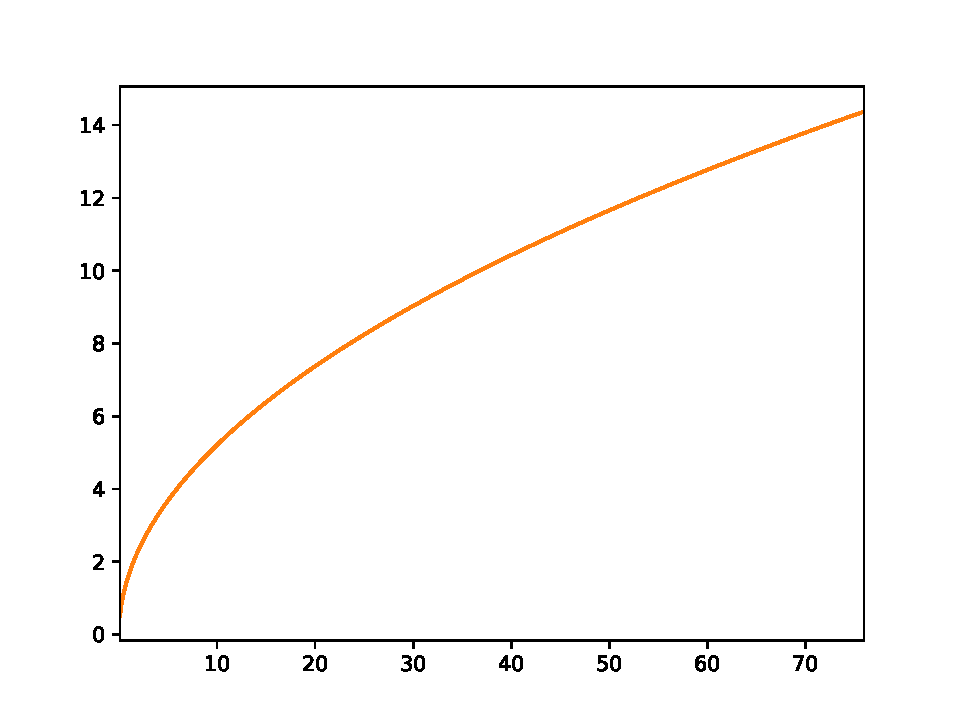
\includegraphics[scale=0.5]
    {\FigDir/ray1.pdf}
    \caption{Aggregate Savings as a Function of Aggregate Market Resources}
    \label{fig:agg_savings}
  \end{figure}

    \begin{figure}[H]
      \centering
        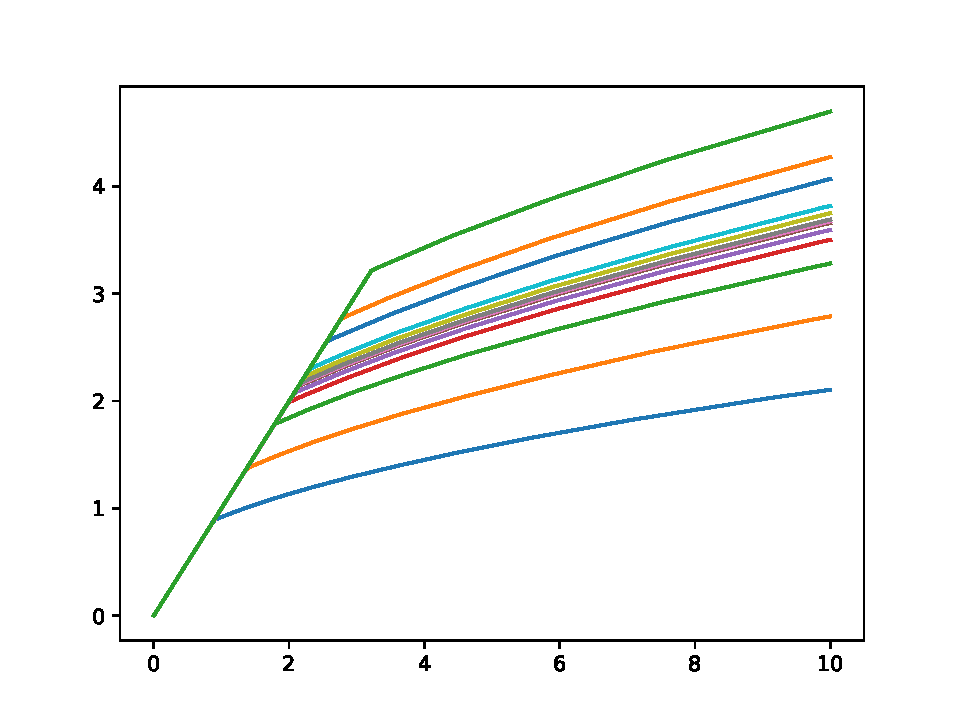
\includegraphics[scale=0.5]{\FigDir/ray3.pdf}
        \caption{Consumption Function at Each Aggregate Market Resources Gridpoint in the Good State}
    \label{fig:good_consumption}
  \end{figure}

Using the same parameters as Krusell and Smith, we managed to produce a similar consumption function using our model as the Krusell-Smith REMARK as shown in Figure \ref{fig:good_consumption}. This result indicates that our model is behaving properly and is pointing in the right direction.  
  
    \begin{figure}[H]
      \centering
        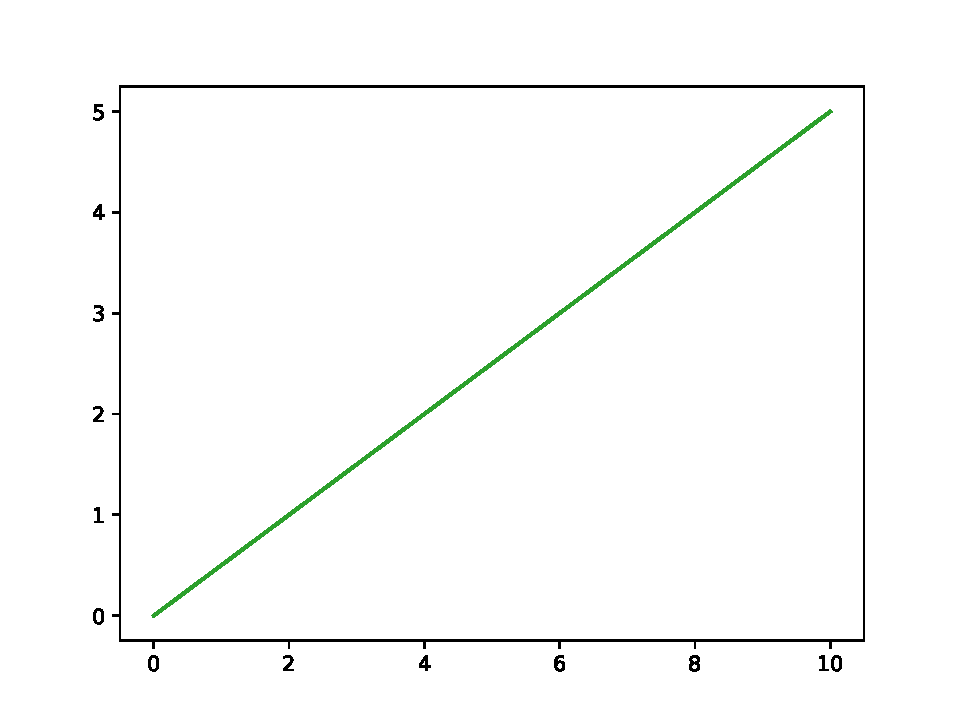
\includegraphics[scale=0.5]{\FigDir/ray2.pdf}
        \caption{Consumption Function at Each Aggregate Market Resources Gridpoint in the Bad State}
    \label{fig:bad_consumption}
  \end{figure}

Unfortunately, consumption function in the bad state is linear and equal across the different market economy grids (M) as shown in Figure \ref{fig:bad_consumption}. Our hypothesis is that following $\texttt{ConsLabrModel}$, zero transitory shock (bad state idiosyncratic shock) causes the end of period marginal value function to become zero which subsequently turns consumption to infinity. In order to avoid this, we forced consumption to be equal to the bank balances grid (b) that  is equal across every market economy grid. 

The reason why we could not make our consumption equal to bank balances in that period is due to the fact that the bank balance in this period is calculated after we have calculated optimal consumption in the current period.


\begin{figure}[H]
      \centering
      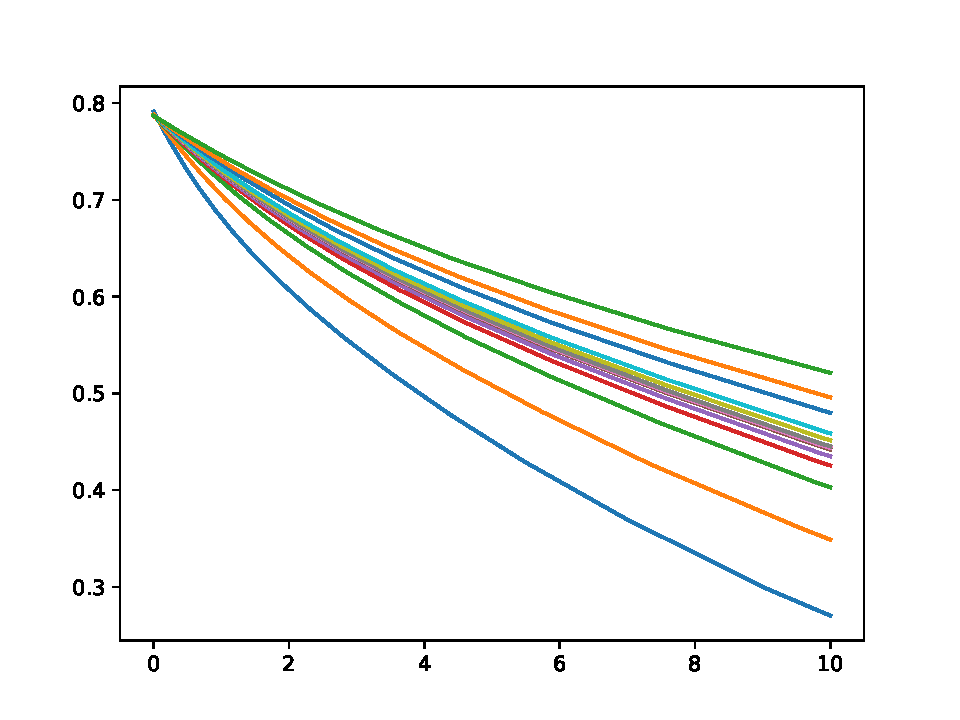
\includegraphics[scale=0.5]
      {\FigDir/ray5.pdf}
      \caption{Labor Function at Each Aggregate Market Resources Gridpoint in the Good State}
    \label{fig:labor_good}
  \end{figure}

As shown in Figure \ref{fig:labor_good} our model was also able to produce a labor function graph that is largely similar to the $\texttt{ConsLabrModel}$ example provided by the econ-ark project accentuating the belief that our model is working correctly. 

  \begin{figure}[H]
        \centering
      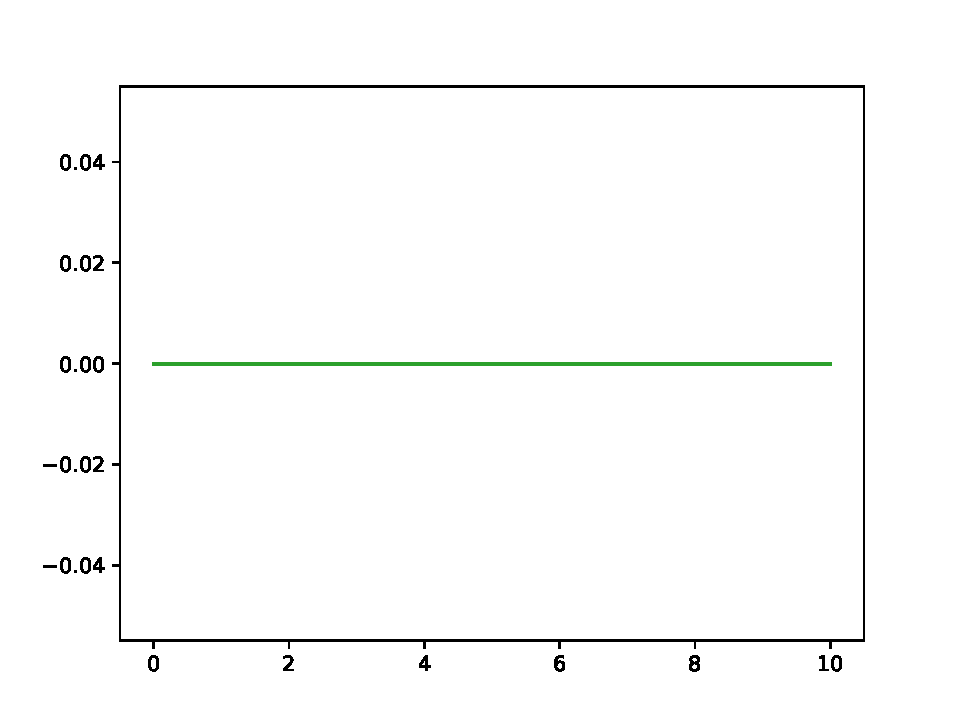
\includegraphics[scale=0.5]
      {\FigDir/ray4.pdf}
      \caption{Labor Function at Each Aggregate Market Resources Gridpoint in the Bad State}
    \label{fig:labor_bad}
  \end{figure}

Finally, Figure \ref{fig:labor_bad} shows the labor function graph during the bad state from our model. Given that labor supply is restricted to zero during bad states, we can see that the labor function is a horizontal line at zero.


\clearpage\pagebreak\vfill\eject

\bibliography{ChangKim-LaborWedge,ChangKim-LaborWedge-Add}\end{document}
